\section{Jump Points By Example}
\label{cha::jps::jumppoints}
The intutition for Jump Point Search is simple: in the process of searching
for an optimal path on a grid map we will aim to selectively expand only
certain ``important'' nodes and ignore all the rest.
We term these important nodes \emph{jump points} and give an example of the 
basic idea in Figure \ref{fig::jps::jumppoints}(a).

When expanding $x$ we may notice that there is little point to evaluating any
neighbour reachable by a dashed line as such a move is always
dominated by (i.e. no better than) an alternative path which mentions 
$p(x)$ but not $x$.
We will make this idea more precise in Section~\ref{cha::jps::pruning} but for now it is 
sufficient to observe that the only non-dominated neighbour of $x$ 
lies immediately to the right.
Rather than generating this neighbour and adding it to the open list,
as in the classical A* algorithm, we propose 
to simply step to the right and continue moving in this direction until we
encounter a node such as $y$; which has at least one other non-dominated
neighbour (here $z$). 
If we find a node such as $y$ (a jump point) we generate it as a successor 
of $x$ and assign it a $g$-value (or cost-so-far) of $g(y) = g(x) + dist(x,
y)$.
Alternatively, if we reach an obstacle we conclude that further search in this
direction is fruitless and generate nothing.
\par
Figure~\ref{fig::jps::jumppoints}(a) is an example of a jump that is based
only on straight moves. In the remainder of this chapter we will develop  
a macro-step operator which is also applicable in the case where the $x$ is reached
from $p(x)$ by a diagonal move. This latter procedure is illustrated in 
Figure~\ref{fig::jps::jumppoints}(b). It is similar in spirit to the previous example;
the main difference is that before each diagonal step we must ensure that the node 
being skipped cannot be a possible turning point for any optimal path. 
We explain this process in more detail in Section~\ref{cha::jps::pruning} when we encapsulate
the process of jumping from one node to another in two simple pruning rules.
One rule is applicable to straight moves, the other diagonal moves.
The purpose of each rule is to decide whether a node should be generated or skipped. 
With these rules in hand we will proceed to give a detailed description of the Jump
Point Search algorithm. We also give a corresponding theoretical result that shows 
that the process of ``jumping over'' nodes has no effect on the optimality of search.

\begin{figure}[tb]
\centering
\begin{minipage}[tb]{0.49\columnwidth}
		   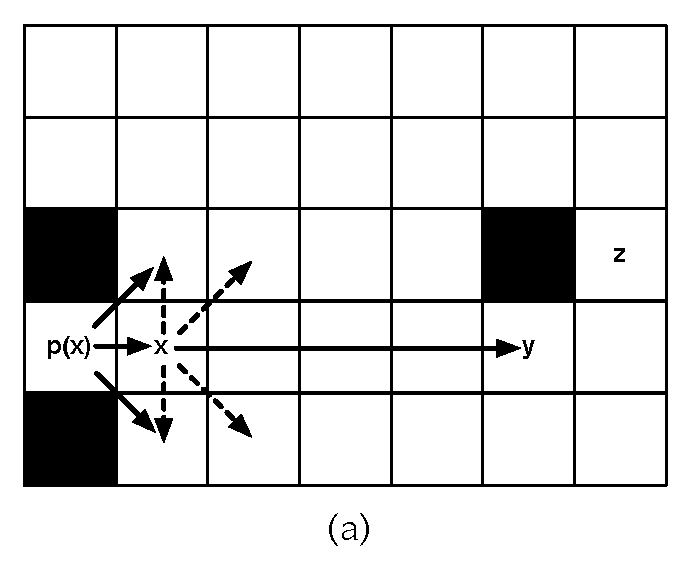
\includegraphics[width=\columnwidth, trim = 4mm 0mm 0mm 0mm]
			{chapter_jps/diagrams/jump_straight.pdf}
\label{fig::jps::jump_straight}
%\caption{Foo}
\end{minipage}
\begin{minipage}[tb]{0.49\columnwidth}
		   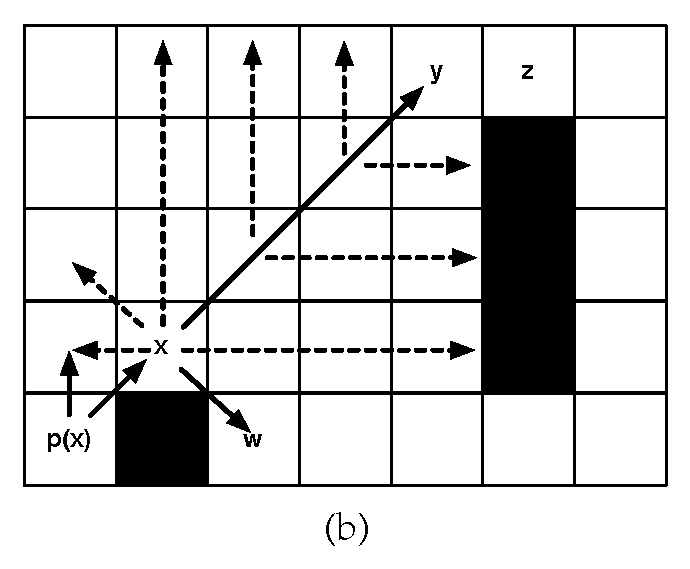
\includegraphics[width=\columnwidth, trim = 0mm 0mm 4mm 0mm]
			{chapter_jps/diagrams/jump_diagonal.pdf}
\label{fig::jps::jump_straight}
%\caption{Bar}
\end{minipage}
\label{fig::jps::jumppoints}
\vspace{-2em}
\caption{Examples of straight jump (a) and a diagonal jump (b).
In both cases the current search is expanding node $x$ with parent node $p(x)$.
Strong straight lines leading away from $x$ indicate successor nodes that are 
considered jump points.
Dashed lines indicate a sequence of interim node evaluations that do not yield any
jump point successors. Strong lines indicate eventual successor nodes.}
\label{fig::jps::jumppoints}
\end{figure}
